% !TEX root = thesis.tex
\documentclass[11pt, % MIT requirements, at least 11 pt
            %    draft,
            %    draftversion, % prints draft on front page
               twoside,
               letterpaper,openright]{mitthesis}

\hypersetup{
  pdfinfo={
    Title={Some long title about some interesting subject},
    Author={John Doe},
    Subject={PhD Thesis},
    Keywords={MIT, some interesting subject}
  }
}

\author{John Doe}

% !TEX root = proposal.tex

% For packages not directly related to MIT thesis class

%%%   Todo notes
\usepackage{xargs}                      % Use more than one optional parameter in a new commands
\usepackage[colorinlistoftodos,prependcaption,textsize=tiny]{todonotes}
\newcommandx{\unsure}[2][1=]{\todo[linecolor=red,backgroundcolor=red!25,bordercolor=red,#1]{#2}}
\newcommandx{\karen}[2][1=]{\todo[linecolor=blue,backgroundcolor=blue!25,bordercolor=blue,#1]{#2}}
\newcommandx{\info}[2][1=]{\todo[linecolor=OliveGreen,backgroundcolor=OliveGreen!25,bordercolor=OliveGreen,#1]{#2}}
\newcommandx{\improvement}[2][1=]{\todo[linecolor=greenc,backgroundcolor=greenc!25,bordercolor=greenc,#1]{#2}}
\newcommandx{\thiswillnotshow}[2][1=]{\todo[disable,#1]{#2}}
% ---------------------------------------------------------------------- %

%%%   Extra commands
%%    Partials
\newcommand{\PDer}[2]{%
    \frac{\partial #1}{\partial #2}
}
\newcommand{\PDerT}[2]{%
    \frac{\partial^2 #1}{\partial #2^2}
}
\newcommand{\PDerF}[2]{%
    \frac{\partial^4 #1}{\partial #2^4}
}
\newcommand{\PDerFM}[3]{%
    \frac{\partial^4 #1}{\partial #2^2 \partial #3^2}
}
\newcommand{\PDerTh}[2]{%
    \frac{\partial^3 #1}{\partial #2^3}
}
\newcommand{\PDerThM}[3]{%
    \frac{\partial^3 #1}{\partial #2 \partial #3}
}

\newcommand{\PDerM}[3]{%
    \frac{\partial^2 #1}{\partial #2 \partial #3}
}
\newcommand{\DerF}[2]{%
    \frac{\mathrm{d}^4 #1}{\mathrm{d} #2^4}
}
\newcommand{\Der}[2]{%
    \frac{\mathrm{d} #1}{\mathrm{d} #2}
}
\newcommand{\DerT}[2]{%
    \frac{\mathrm{d}^2 #1}{\mathrm{d} #2^2}
}
\newcommand{\DerTh}[2]{%
    \frac{\mathrm{d}^3 #1}{\mathrm{d} #2^3}
}

%% Extra math commands
\newcommand*{\rttensor}[1]{\overline{\overline{#1}}}
\newcommand{\bomega}{\textrm{\boldmath$\omega$}}
\DeclareMathOperator*{\argmin}{arg\,min}
\DeclareMathOperator{\Tr}{Tr}

%%% Tikz
%%  3D Plot
\makeatletter
\tikzoption{canvas is xy plane at z}[]{%
  \def\tikz@plane@origin{\pgfpointxyz{0}{0}{#1}}%
  \def\tikz@plane@x{\pgfpointxyz{1}{0}{#1}}%
  \def\tikz@plane@y{\pgfpointxyz{0}{1}{#1}}%
  \tikz@canvas@is@plane
}
\makeatother

% checkmarks etc.
\definecolor{darkgreen}{RGB}{26, 139, 26}
\newcommand{\Cross}{$\mathbin{\tikz [x=1.4ex,y=1.4ex,line width=.2ex, MITred] \draw (0,0) -- (1,1) (0,1) -- (1,0);}$}%
\newcommand{\Checkmark}{$\color{darkgreen}\checkmark$}

\newcommand{\todofig}{%
  \begin{tikzpicture}%
    \draw[line cap=rect,fill=MITred!50] (0,0) rectangle (\linewidth-\pgflinewidth,-5) node[pos=.5] {WORK IN PROGRESS};
  \end{tikzpicture}
}

%%% Nomenclature

% Copying \! to \negspace -- can't use \! in nomenclature
\let\negspace\!

\usepackage{nomencl}
\usepackage{etoolbox,ragged2e,mathtools} % Nomenclature

\DeclarePairedDelimiter{\abs}{\lvert}{\rvert}
\setlength{\nomitemsep}{-\parsep}
\addtolength{\nomitemsep}{4pt} % same as list of figures/tables

\renewcommand{\nomgroup}[1]{\medskip}

\renewcommand*{\nompreamble}{\markboth{\nomname}{\nomname}}
\renewcommand{\nomname}{Nomenclature}

\makenomenclature

%%% Equations

% cancel parts of equation
\usepackage{cancel}

\newcommand{\crit}{\textrm{crit}}
\newcommand{\fl}{\textrm{fl}}
\newcommand{\eng}{\textrm{eng}}
\newcommand{\smc}{\textrm{smc}}
\newcommand{\overbar}[1]{\mkern 1.5mu\overline{\mkern-1.5mu#1\mkern-0.75mu}\mkern 0.75mu}

% Transpose symbol
\newcommand{\trans}{\mathsf{\mathsmaller T}}

% To gray out zeros
\newcommand{\zz}{\textcolor{gray!75}{\mathbf{0}}}
\newcommand{\zzs}{\textcolor{gray!75}{0}}

\newcommand{\enn}{n}
\newcommand{\emm}{m}

%%% Acronyms
%%% Flutter
\newacronym{cfd}{cfd}{Computational Fluid Dynamics}
\newacronym{naca}{naca}{National Advisory Committee for Aeronautics}
\newacronym{fem}{fem}{Finite Element Method}


%%% Fonts

% special commands for lining figures
\newcommand{\SUTwo}{{\myliningnumfont SU2}}
\newcommand{\RAE}{{\myliningnumfont RAE2822}}
\newcommand{\NACASIX}{{\myliningnumfont NACA64A010}}
\newcommand{\TwoD}{{\myliningnumfont 2D}}
\newcommand{\ThreeD}{{\myliningnumfont 3D}}
\newcommand{\DTwo}{{\myliningnumfont D8.2}}
\newcommand{\DZero}{{\myliningnumfont D8.0}}
\newcommand{\NThree}{{\myliningnumfont N+3}}

% Hyphenation
\hyphenation{mecan-ique}
\hyphenation{Helm-holtz}

\usepackage{lipsum} % filler material


\addbibresource{bibliography.bib}

\begin{document}
  \chapterstyle{mit}
  \pagestyle{mit}
  \maxsecnumdepth{subsection}

    \mainmatter

      \begin{whole}
        \maketitle
      \end{whole}

      {\pagestyle{plain}%
      \printabstract{chapters/0_abstract}%
      }
      \cleardoublepage

      {%
\thispagestyle{empty}%
\begin{vplace}[0.7]
\mbox{}\hfill This thesis is dedicated to \vspace{1pc}\\
\mbox{}\hfill {\large .....}
\end{vplace}%
}


      \cleardoublepage
      \pdfbookmark[chapter]{Acknowledgements}{acknowledgements}%

\chapter*{Acknowledgements}


\lipsum[1]
Thank you! \\

\vspace{1em}
\mbox{} \hfill \textit{Author}\\
\mbox{} \hfill Cambridge, Massachusetts\\
\mbox{} \hfill August 2025


      \cleardoublepage%
      \pdfbookmark{\contentsname}{toc}%
      \tableofcontents*

      \cleardoublepage

      {\phantomsection%
      % Just put it in a random order, it will be ordered automatically

%%% Roman

% 3D flutter
\nomenclature[$V$]{$\mathbf{V}$}{Velocity field}
\nomenclature[$V_{\infty}$]{$V_{\negspace\infty}$}{Freestream velocity}

%%% Greek

% 2D flutter
\nomenclature[g$\alpha$]{$\alpha$}{Angle of attack}
\nomenclature[g$\rho$]{$\rho_{\infty}$}{Freestream density}
%
      \addcontentsline{toc}{chapter}{Nomenclature}%
      \printnomenclature[0.8in]%
      }%

      \cleardoublepage

      {\phantomsection%
      \printglossary[title=Acronyms,type=\acronymtype]}

      \cleardoublepage

      {\RaggedRight\listoffigures\cleardoublepage
      \listoftables}

      % !TEX root = ../thesis.tex
\chapter{Introduction}\label{chap:intro}

\textit{Some fear flutter because they do not understand it.}\\
\textit{And some fear it because they do.} \vspace{5pt} \\
--- Theodore von K\'arm\'an \\

\noindent \lipsum[3-8]


      % !TEX root = ../thesis.tex
\chapter{Methods}\label{chap:methods}

This
\published{Part of the research presented in this chapter has been published as\\ \textit{Doe J., \href{http://dx.doi.org/10.2514/1.J056710}{\mkbibquote{Some interesting journal paper,}}} AIAA Journal,  \textit{Vol. 56, No. 4, 2018, pp. 1519–1531.} }%
chapter discusses something. \lipsum[1]

\begin{figure}[ht]
   \begin{fullwidthfig}
     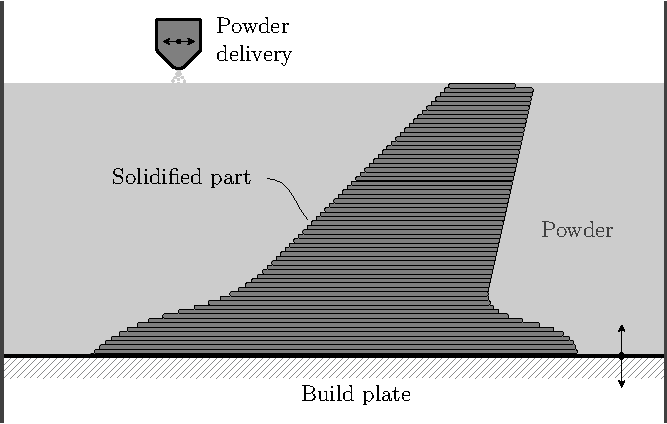
\includegraphics[width=0.9\fullwidth]{figures/example/powder_based}
   \end{fullwidthfig}
   \captionb[Shorter caption for in the LOF.]{This is some exciting figure, generated in Tikz. Note how the caption is below the figure.}{fig:tikz}
\end{figure}

 \lipsum[2]

 \begin{figure}[ht]
   \begin{sidecaption}[Some temporary figure.]{This will eventually have some exciting figure. Note how the caption is alongside the figure}[fig:temp]
     \todofig
   \end{sidecaption}
 \end{figure}

Now we are adding some citations next to the body of the text.\mcite{drela1999integrated,theodorsen1935general,weissinger_naca}
\lipsum[3]
Down the line, if you cite the same article again, the number is repeated.\mcite{drela1999integrated}
If you click the number in the text, you are taken to the bibliography---same for clicking the number of the sidenote.
If you click the title of the article in the margin, you are taken to article itself (through the DOI, ISBN, or website in the bibliography)---same for clicking the title in the bibliography itself.
If you click the number in ``cited on...'' in the bibliography's margin, you are taken back to the text where the article was cited.

Finally, you can also add sidenotes to the text, like so.\sidenote{Some interesting tidbit of information that was not important enough for the main text.}
Please \textit{do not} use footnotes.


      % !TEX root = ../thesis.tex
\chapter{Results}\label{chap:results}

\lipsum[1-8]


      % !TEX root = ../thesis.tex
\chapter{Conclusions and Outlook}\label{chap:conclusion}

This thesis presented some stuff.
\lipsum[9-15]


      \printbibliography

      \addcontentsline{toc}{part}{\appendixtocname}
      \appendixpage*

      \def\chaptername{Appendix}

      \bookmarksetup{startatroot}
      \appendix
      % !TEX root = ../thesis.tex
\chapter{Some stuff that was not important enough}\label{app:app}

\lipsum[8-10]


      {\small\printindex}

      \newpage  \clearpage \mbox{}
      {%
\thispagestyle{empty}%
\small%
\vfill%
\pdfbookmark[chapter]{Colophon}{colophon}%
\section*{Colophon}
% \noindent This thesis has been typeset using \LaTeX{} in the Palatino font.
\noindent This thesis has been typeset using \LaTeX{}, and compiled using \texttt{pdflatex}.
Minion Pro is used as both the text and display typeface.
The sans-serif text uses the \textsf{Myriad Pro} typeface, whereas monospaced text is typeset in \texttt{Bitstream Vera Mono}.
Line figures and illustrations were predominantly generated  using the \href{https://ctan.org/pkg/pgf?lang=en}{Tikz} \LaTeX{} package, \acrshort{fem} data plots using \href{https://www.tecplot.com/}{Tecplot}, and renders using \href{https://www.blender.org/}{Blender}.
\mbox{}\vspace{0.5pc}\\
\noindent Several books have influenced the style, typography, and graphic design of this thesis, in particular:
\begin{itemize}
  \item[] Edward Tufte's \textit{Beautiful Evidence} (2006)
  \item[] Jean-Luc Doumont's \textit{Trees, Maps, and Theorems} (2009)
  \item[] Robert Bringhurst's \textit{Elements of Typography} (1992)
\end{itemize}
\vspace{0.75pc}% \mbox{}\\

\noindent\textit{Very Long }\\
\textit{thesis title}\vspace{0.25pc}\\
Author, September 2018 \vspace{1.25pc}\\
\noindent \textcopyright\ Massachusetts Institute of Technology 2018. All rights reserved.\vspace{1pc} \\
}


      \newpage  \clearpage \mbox{} \thispagestyle{empty}
      \newpage  \clearpage \mbox{} \thispagestyle{empty}%
      {%
        \begin{tikzpicture}[remember picture,overlay]
        \node[at=(current page.south),gray,anchor=south,yshift=1in,text width=0.5\paperwidth,align=center]{
            \footnotesize%
            \begin{minipage}{\linewidth}
                  \centering
                  Ph.D. Dissertation\\
                  John Doe\vskip0.5em
                  \textit{Some very long title}\\
                  \textit{about some interesting topic}\vskip0.5em
                  -- \textsc{mmxviii} --
            \end{minipage}};
        \end{tikzpicture}
      }

\end{document}
